\let\negmedspace\undefined
\let\negthickspace\undefined
\documentclass[journal]{IEEEtran}
\usepackage[a5paper, margin=10mm, onecolumn]{geometry}
\usepackage{lmodern} % Ensure lmodern is loaded for pdflatex
\usepackage{tfrupee} % Include tfrupee package

\setlength{\headheight}{1cm} % Set the height of the header box
\setlength{\headsep}{0mm}  % Set the distance between the header box and the top of the text
\usepackage{romannum}
\usepackage{tfrupee}
\usepackage{csquotes}
\usepackage{gvv-book}
\usepackage{gvv}
\usepackage{circuitikz}
\usepackage{cite}
\usepackage{float}
\usepackage{amsmath,amssymb,amsfonts,amsthm}
\usepackage{algorithmic}
\usepackage{graphicx}
\usepackage{textcomp}
\usepackage{xcolor}
\usepackage{txfonts}
\usepackage{listings}
\usepackage{enumitem}
\usepackage{mathtools}
\usepackage{gensymb}
\usepackage{comment}
\usepackage[breaklinks=true]{hyperref}
\usepackage{tkz-euclide} 
\usepackage{listings}
% \usepackage{gvv}                                        
\def\inputGnumericTable{}                                 
\usepackage[latin1]{inputenc}                                
\usepackage{color}                                            
\usepackage{array}                                            
\usepackage{longtable}                                       
\usepackage{calc}                                             
\usepackage{multirow} 
\usepackage{multicol}
\usepackage{hhline}   
\usepackage{enumitem}
\usepackage{ifthen}                                           
\usepackage{lscape}
\usepackage{caption}
\usepackage{tikz}
\usetikzlibrary{patterns}

\title{GATE 2025 Question Paper (Life Sciences - XL)}
\author{EE25BTECH11019 \\ Vivek Darji}
\date{}

\begin{document}

\maketitle
\section*{General Aptitude (GA)}
\begin{enumerate}

    \item Even though I had planned to go skiing with my friends, I had to \underline{\rule{2cm}{0pt}} at the last moment because of an injury.

    \hfill{\brak{\text{GATE XL 2025}}}

    \begin{enumerate}
        \begin{multicols}{4}
            \item back up
            \item back of
            \item back on
            \item back out
        \end{multicols}
    \end{enumerate}

    \item The President, along with the Council of Ministers, \underline{\rule{2cm}{0pt}} to visit India next week.

    \hfill{\brak{\text{GATE XL 2025}}}

    \begin{enumerate}
        \begin{multicols}{4}
            \item will visit
            \item will wish
            \item is visiting
            \item is wishing
        \end{multicols}
    \end{enumerate}

    \item An electricity utility company charges \rupee $7$ per kWh \brak{\text{kilo watt-hour}}. If a $40$-watt desk light is left on for $10$ hours each night for $180$ days, what would be the cost of energy consumption? If the desk light is on for $2$ more hours each night for the $180$ days, what would be the percentage-increase in the cost of energy consumption?

    \hfill{\brak{\text{GATE XL 2025}}}

    \begin{enumerate}
        \begin{multicols}{2}
            \item \rupee $604.8$; $10\%$
            \item \rupee $504$; $20\%$
            \item \rupee $604.8$; $12\%$
            \item \rupee $720$; $15\%$
        \end{multicols}
    \end{enumerate}

    \item In the context of the given figure, which one of the following options correctly represents the entries in the blocks labelled \brak{\text{i}}, \brak{\text{ii}}, \brak{\text{iii}}, and \brak{\text{iv}}, respectively?

    \begin{figure}[H]
        \centering
        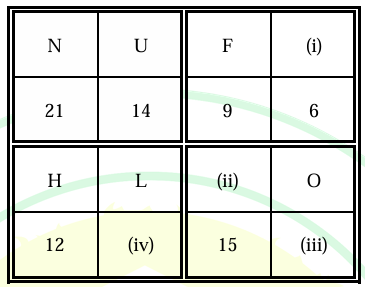
\includegraphics[width=0.8\columnwidth]{figs/q4.png}
        \caption*{}
        \label{fig:q4}
    \end{figure}

    \hfill{\brak{\text{GATE XL 2025}}}

    \begin{enumerate}
        \begin{multicols}{2}
            \item Q, M, $12$, and $8$
            \item K, L, $10$ and $14$
            \item I, J, $10$, and $8$
            \item L, K, $12$ and $8$
        \end{multicols}
    \end{enumerate}

    \item A bag contains Violet \brak{\text{V}}, Yellow \brak{\text{Y}}, Red \brak{\text{R}}, and Green \brak{\text{G}} balls. On counting them, the following results are obtained\brak{\text{:}}\\
    \brak{\text{i}} The sum of Yellow balls and twice the number of Violet balls is $50$.\\
    \brak{\text{ii}} The sum of Violet and Green balls is $50$.\\
    \brak{\text{iii}} The sum of Yellow and Red balls is $50$.\\
    \brak{\text{iv}} The sum of Violet and twice the number of Red balls is $50$.\\
    Which one of the following Pie charts correctly represents the balls in the bag?

    \hfill{\brak{\text{GATE XL 2025}}}

    \begin{figure}[H]
        \centering
        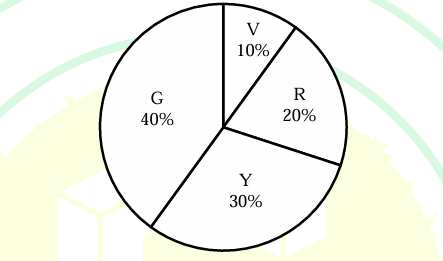
\includegraphics[width=0.45\columnwidth]{figs/a38a.png}
        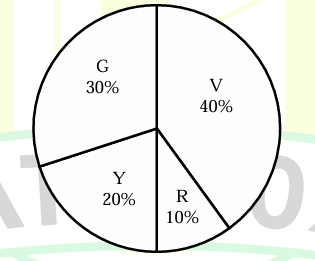
\includegraphics[width=0.45\columnwidth]{figs/a38b.png}\\
        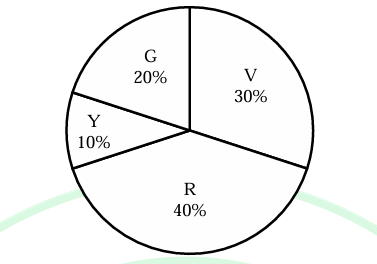
\includegraphics[width=0.45\columnwidth]{figs/a38c.png}
        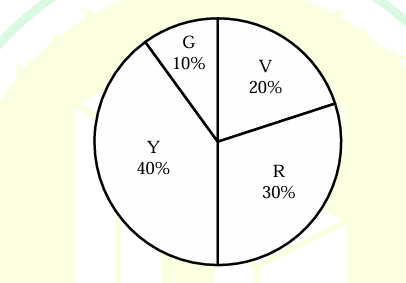
\includegraphics[width=0.45\columnwidth]{figs/a38d.png}
        \caption*{}
        \label{fig:q5_options}
    \end{figure}

    \item ``His life was divided between the books, his friends, and long walks. A solitary man, he worked at all hours without much method, and probably courted his fatal illness in this way. To his own name there is not much to show; but such was his liberality that he was continually helping others, and fruits of his erudition are widely scattered, and have gone to increase many a comparative stranger's reputation.'' \brak{\text{From E.V. Lucas's ``A Funeral''}} Based only on the information provided in the above passage, which one of the following statements is true?

    \hfill{\brak{\text{GATE XL 2025}}}

    \begin{enumerate}
        \item The solitary man described in the passage is dead.
        \item Strangers helped create a grand reputation for the solitary man described in the passage.
        \item The solitary man described in the passage found joy in scattering fruits.
        \item The solitary man worked in a court where he fell ill.
    \end{enumerate}

    \item For the clock shown in the figure, if $O = OQSZPRT$, and $X = XZPWYOQ$, then which one among the given options is most appropriate for $P$?

    \begin{figure}[H]
        \centering
        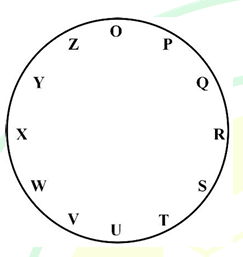
\includegraphics[width=0.8\columnwidth]{figs/q7.png}
        \caption*{}
        \label{fig:q7}
    \end{figure}

    \hfill{\brak{\text{GATE XL 2025}}}

    \begin{enumerate}
        \begin{multicols}{2}
            \item PUWRTVX
            \item PRTOQSU
            \item PTVQSUW
            \item PSUPRTV
        \end{multicols}
    \end{enumerate}

    \item Consider a five-digit number $PQRST$ that has distinct digits $P, Q, R, S,$ and $T$, and satisfies the following conditions\brak{\text{:}} $P < Q$, $S > P > T$, $R < T$. If integers $1$ through $5$ are used to construct such a number, the value of $P$ is

    \hfill{\brak{\text{GATE XL 2025}}}

    \begin{enumerate}
        \begin{multicols}{4}
            \item $1$
            \item $2$
            \item $3$
            \item $4$
        \end{multicols}
    \end{enumerate}

    \item A business person buys potatoes of two different varieties $P$ and $Q$, mixes them in a certain ratio and sells them at \rupee $192$ per kg. The cost of the variety $P$ is \rupee $800$ for $5$ kg. The cost of the variety $Q$ is \rupee $800$ for $4$ kg. If the person gets $8\%$ profit, what is the $P \colon Q$ ratio \brak{\text{by weight}}?

    \hfill{\brak{\text{GATE XL 2025}}}

    \begin{enumerate}
        \begin{multicols}{4}
            \item $5 \colon 4$
            \item $3 \colon 4$
            \item $3 \colon 2$
            \item $1 \colon 1$
        \end{multicols}
    \end{enumerate}

    \item Three villages $P$, $Q$, and $R$ are located in such a way that the distance $PQ = 13\,\text{km}$, $QR = 14\,\text{km}$, and $RP = 15\,\text{km}$, as shown in the figure. A straight road joins $Q$ and $R$. It is proposed to connect $P$ to this road $QR$ by constructing another road. What is the minimum possible length \brak{\text{in km}} of this connecting road?

    \begin{figure}[H]
        \centering
        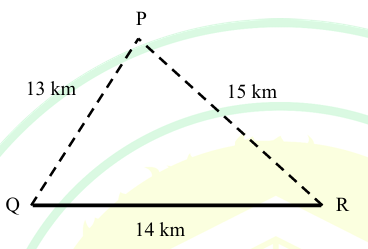
\includegraphics[width=0.8\columnwidth]{figs/q10.png}
        \caption*{}
        \label{fig:q10}
    \end{figure}

    \hfill{\brak{\text{GATE XL 2025}}}

    \begin{enumerate}
        \begin{multicols}{4}
            \item $10.5$
            \item $11.0$
            \item $12.0$
            \item $12.5$
        \end{multicols}
    \end{enumerate}

\section*{Q. 11 - Q. 19 carry one mark each.}

    \item The rate of solvolysis for the following tertiary halides in $80\%$ aqueous ethanol at $25\,\degree$C follows the order

    \begin{figure}[H]
        \centering
        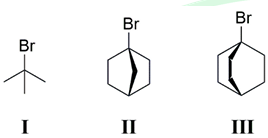
\includegraphics[width=0.8\columnwidth]{figs/xl2025_q11_que.png}
        \caption*{Q11 que.}
        \label{fig:xl2025_q11_que}
    \end{figure}

    \hfill $\brak{\text{GATE XL 2025}}$

    \begin{enumerate}
        \begin{multicols}{2}
            \item I $<$ II $<$ III
            \item II $<$ III $<$ I
            \item III $<$ II $<$ I
            \item II $<$ I $<$ III
        \end{multicols}
    \end{enumerate}

    \item The CORRECT order of boiling points for the hydrogen halides is

    \hfill $\brak{\text{GATE XL 2025}}$

    \begin{enumerate}
        \begin{multicols}{2}
            \item HF $>$ HI $>$ HBr $>$ HCl
            \item HF $>$ HCl $>$ HBr $>$ HI
            \item HI $>$ HBr $>$ HCl $>$ HF
            \item HI $>$ HF $>$ HBr $>$ HCl
        \end{multicols}
    \end{enumerate}

    \item The bond order in $\text{N}_2^-$ species is

    \hfill $\brak{\text{GATE XL 2025}}$

    \begin{enumerate}
        \begin{multicols}{4}
            \item $2$
            \item $2.5$
            \item $3$
            \item $3.5$
        \end{multicols}
    \end{enumerate}

    \item The standard enthalpy of the reaction, C $\brak{\text{graphite}}$ + H$_2$O $\brak{\text{g}}$ $\rightarrow$ CO $\brak{\text{g}}$ + H$_2$ $\brak{\text{g}}$ is found to be $+131.3$ kJ mol$^{-1}$ and the $\Delta_f H^\circ$ value for CO $\brak{\text{g}}$ is $-110.5$ kJ mol$^{-1}$. The value of $\Delta_f H^\circ$ $\brak{\text{in kJ mol}^{-1}}$ for H$_2$O $\brak{\text{g}}$ is

    \hfill $\brak{\text{GATE XL 2025}}$

    \begin{enumerate}
        \begin{multicols}{2}
            \item $+241.8$
            \item $-241.8$
            \item $+20.8$
            \item $-20.8$
        \end{multicols}
    \end{enumerate}

    \item The temperature dependence of reaction rates is generally given by the Arrhenius equation. A plot of $\ln k_r$ against $1/T$ is a straight line from which the pre-exponential factor $A$ and the activation energy $E_a$ can be determined. The CORRECT option regarding this plot is

    \hfill $\brak{\text{GATE XL 2025}}$

    \begin{enumerate}
        \item Slope: $-\dfrac{E_a}{R}$; Intercept on the $y$-axis: $\ln A$
        \item Slope: $+\dfrac{E_a}{2.303R}$; Intercept on the $y$-axis: $A$
        \item Slope: $+\dfrac{E_a}{R}$; Intercept on the $y$-axis: $A$
        \item Slope: $-\dfrac{E_a}{2.303R}$; Intercept on the $y$-axis: $\ln A$
    \end{enumerate}

    \item The isothermal expansion of one mole of an ideal gas from $V_i$ to $V_f$ at temperature $T$ occurs in two ways.\\
    Path I: a reversible isothermal expansion;\\
    Path II: free expansion against zero external pressure.\\
    The CORRECT option for the values of $\Delta U$, $q$ and $w$ for Path I and Path II is

    \hfill $\brak{\text{GATE XL 2025}}$

    \begin{enumerate}
        \item Path I: $\Delta U = 0$, $q > 0$, $w < 0$\\
              Path II: $\Delta U = 0$, $q = 0$, $w = 0$
        \item Path I: $\Delta U = 0$, $q > 0$, $w < 0$\\
              Path II: $\Delta U > 0$, $q > 0$, $w = 0$
        \item Path I: $\Delta U = 0$, $q < 0$, $w > 0$\\
              Path II: $\Delta U = 0$, $q > 0$, $w < 0$
        \item Path I: $\Delta U = 0$, $q < 0$, $w > 0$\\
              Path II: $\Delta U < 0$, $q = 0$, $w = 0$
    \end{enumerate}

    \item The CORRECT statement(s) regarding the given molecules is(are)

    \begin{figure}[H]
        \centering
        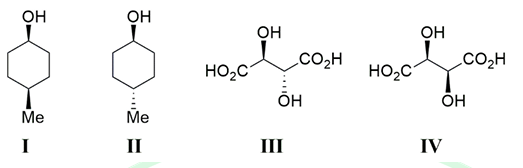
\includegraphics[width=0.8\columnwidth]{figs/xl2025_q17_que.png}
        \caption*{Q17 que.}
        \label{fig:xl2025_q17_que}
    \end{figure}

    \hfill $\brak{\text{GATE XL 2025}}$

    \begin{enumerate}
        \item Both I and II are achiral molecules.
        \item Both II and III are chiral molecules.
        \item IV is a chiral molecule.
        \item Both III and IV are chiral molecules.
    \end{enumerate}

    \item The CORRECT statement(s) about $\brak{\text{[Ni(CN)}_4\text{]}^{2-}}$, $\brak{\text{[Ni(CO)}_4\text{]}}$ and $\brak{\text{[NiCl}_4\text{]}^{2-}}$ is(are)\\
    $\brak{\text{Given: Atomic number of Ni: 28}}$

    \hfill $\brak{\text{GATE XL 2025}}$

    \begin{enumerate}
        \item $\brak{\text{[Ni(CN)}_4\text{]}^{2-}}$ is diamagnetic and $\brak{\text{[NiCl}_4\text{]}^{2-}}$ is paramagnetic.
        \item Both $\brak{\text{[Ni(CO)}_4\text{]}}$ and $\brak{\text{[NiCl}_4\text{]}^{2-}}$ are paramagnetic.
        \item $\brak{\text{[Ni(CN)}_4\text{]}^{2-}}$ is square planar and $\brak{\text{[NiCl}_4\text{]}^{2-}}$ is tetrahedral in shape.
        \item All three complexes are paramagnetic.
    \end{enumerate}

    \item Consider the two pKa values of valine as $2.32$ and $9.62$. The isoelectric point $\brak{\text{pI}}$ of this amino acid is $\underline{\rule{2cm}{0pt}}$ (rounded off to two decimal places).

    \hfill $\brak{\text{GATE XL 2025}}$

\section*{Q. 20 - Q. 27 carry two marks each.}

    \item A few species are given in Column I. Column II contains the hybrid orbitals used by the central atom of the species for bonding. The CORRECT match for the species to their central atom hybridization is\\
    $\brak{\text{Given: Atomic numbers of B: 5; C: 6; O: 8; F: 9; P: 15; Cl: 17; I: 53}}$

    \hfill $\brak{\text{GATE XL 2025}}$

    \begin{enumerate}
        \item i-d, ii-c, iii-b, iv-a
        \item i-d, ii-b, iii-c, iv-a
        \item i-d, ii-c, iii-a, iv-b
        \item i-c, ii-d, iii-b, iv-a
    \end{enumerate}

    \item For product formation from only one type of reactant $\brak{\text{e.g. A} \rightarrow \text{product}}$, the CORRECT match for the order of the reaction $\brak{\text{given in Column I}}$ with the half-life expression $\brak{\text{given in Column II}}$ is\\
    $\brak{\text{[A]}_0}$ is the initial concentration and $k_r$ is the rate constant

    \hfill $\brak{\text{GATE XL 2025}}$

    \begin{enumerate}
        \item i-R, ii-P, iii-S
        \item i-S, ii-R, iii-Q
        \item i-Q, ii-P, iii-S
        \item i-Q, ii-R, iii-P
    \end{enumerate}

    \item The CORRECT statement(s) for the given reactions is(are)

    \begin{figure}[H]
        \centering
        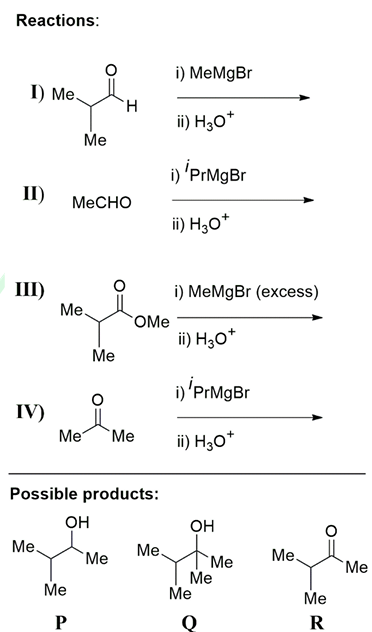
\includegraphics[width=0.8\columnwidth]{figs/xl2025_q22_que.png}
        \caption*{Q22 que.}
        \label{fig:xl2025_q22_que}
    \end{figure}

    \hfill $\brak{\text{GATE XL 2025}}$

    \begin{enumerate}
        \item P is formed as the major product in reaction II.
        \item Q is formed as the major product in reaction IV.
        \item R is formed as the major product in reaction III.
        \item P is formed as the major product in reaction I.
    \end{enumerate}

    \item Addition of a few drops of concentrated HCl to an aqueous solution of CoCl$_2$ forms a dark blue complex X. The CORRECT statement(s) for this reaction is(are)\\
    $\brak{\text{Given: Atomic number of Co: 27}}$

    \hfill $\brak{\text{GATE XL 2025}}$

    \begin{enumerate}
        \item X is a centrosymmetric complex.
        \item The oxidation state of cobalt does not change in this reaction.
        \item The number of unpaired electrons on cobalt in X and in CoCl$_2$ $\brak{\text{aqueous solution}}$ are the same.
        \item The spin only magnetic moment value for X is $3.87$ BM.
    \end{enumerate}

    \item The CORRECT statement(s) regarding biomolecules is(are)

    \hfill $\brak{\text{GATE XL 2025}}$

    \begin{enumerate}
        \item The N-terminal amino acid of a polypeptide can be identified by Edman's reagent $\brak{\text{phenyl isothiocyanate}}$.
        \item L-Threonine has only one chiral center.
        \item Cytosine is present both in RNA and DNA.
        \item A mixture of different amino acids can be separated by ion-exchange chromatography.
    \end{enumerate}

    \item Energy of the transition from $n = 4$ to $n = 2$ for hydrogen atom is $E \times 10^3$ cm$^{-1}$.\\
    $\brak{\text{Given: Rydberg constant for hydrogen: } 1.097 \times 10^7\ \text{m}^{-1}}$\\
    Value of $E$ is $\underline{\rule{2cm}{0pt}}$ (rounded off to two decimal places)

    \hfill $\brak{\text{GATE XL 2025}}$

    \item A non-volatile solute has a molecular weight of $180$ g mol$^{-1}$. Assume that the solute does not associate or dissociate in water, and the boiling-point constant $\brak{\text{ebullioscopic constant}}$ of water is $0.51$ K kg mol$^{-1}$.\\
    The amount $\brak{\text{in g}}$ of solute added to $500$ g of water to elevate the boiling point by $0.153$ K is $\underline{\rule{2cm}{0pt}}$ (answer in integer)

    \hfill $\brak{\text{GATE XL 2025}}$

    \item The standard potentials $\brak{E^\circ}$ for the Fe$^{3+}$/Fe and Fe$^{3+}$/Fe$^{2+}$ couples are $-0.04$ V and $+0.76$ V, respectively.\\
    $\brak{\text{Given: Faraday constant } = 96500\ \text{C mol}^{-1}}$

    \hfill $\brak{\text{GATE XL 2025}}$

\section*{Biochemistry (XL-Q)}
\section*{Q.28 - Q.35 carry one mark each.}

    \item Zinc is essential for the function of

    \hfill $\brak{\text{GATE XL 2025}}$

    \begin{enumerate}
        \begin{multicols}{2}
            \item carboxypeptidase A
            \item chlorophyll a
            \item myoglobin
            \item vitamin B$_{12}$
        \end{multicols}
    \end{enumerate}

    \item Which one of the following molecules captures CO$_2$ in the C$_4$ cycle?

    \hfill $\brak{\text{GATE XL 2025}}$

    \begin{enumerate}
        \begin{multicols}{2}
            \item 1,3-Bisphosphoglycerate
            \item Oxaloacetate
            \item Phosphoenolpyruvate
            \item Ribulose-1,5-bisphosphate
        \end{multicols}
    \end{enumerate}

    \item Which one of the following methods separates biomolecules based on their hydrodynamic volumes?

    \hfill $\brak{\text{GATE XL 2025}}$

    \begin{enumerate}
        \begin{multicols}{2}
            \item Anion-exchange chromatography
            \item Cation-exchange chromatography
            \item Size-exclusion chromatography
            \item Thin-layer chromatography
        \end{multicols}
    \end{enumerate}

    \item Which one of the following restriction endonucleases is a blunt cutter?

    \hfill $\brak{\text{GATE XL 2025}}$

    \begin{enumerate}
        \begin{multicols}{4}
            \item BamHI
            \item EcoRI
            \item HindIII
            \item SmaI
        \end{multicols}
    \end{enumerate}

    \item Which one of the following DNA repair systems requires DNA glycosylases?

    \hfill $\brak{\text{GATE XL 2025}}$

    \begin{enumerate}
        \begin{multicols}{4}
            \item Base-excision
            \item Direct
            \item Mismatch
            \item Nucleotide-excision
        \end{multicols}
    \end{enumerate}

    \item Which one of the following ion channels opens to repolarize the neuronal membrane when an action potential is generated?

    \hfill $\brak{\text{GATE XL 2025}}$

    \begin{enumerate}
        \begin{multicols}{4}
            \item Ca$^{2+}$ channel
            \item H$^+$ channel
            \item Na$^+$ channel
            \item K$^+$ channel
        \end{multicols}
    \end{enumerate}

    \item Which one of the following is the most sensitive immunoassay?

    \hfill $\brak{\text{GATE XL 2025}}$

    \begin{enumerate}
        \begin{multicols}{2}
            \item Immunoelectrophoresis
            \item Immunofluorescence
            \item Radial immunodiffusion
            \item Radioimmunoassay
        \end{multicols}
    \end{enumerate}

    \item Which of the following statements about antibodies is/are correct?

    \hfill $\brak{\text{GATE XL 2025}}$

    \begin{enumerate}
        \item Different antibody classes have different effector functions.
        \item Each antibody chain consists of an amino-terminal constant region and a carboxy-terminal variable region.
        \item Variable domains harbour complementarity-determining regions.
        \item Antibodies are produced only by T cells.
    \end{enumerate}

\section*{Q.36 - Q.46 carry two marks each.}

    \item Which one of the following molecules does NOT contain phosphoanhydride bond(s)?

    \hfill $\brak{\text{GATE XL 2025}}$

    \begin{enumerate}
        \begin{multicols}{2}
            \item Adenosine diphosphate
            \item Adenosine triphosphate
            \item Fructose-1,6-bisphosphate
            \item Pyrophosphate
        \end{multicols}
    \end{enumerate}

    \item For an enzyme that follows Michaelis-Menten kinetics, a competitive inhibitor

    \hfill $\brak{\text{GATE XL 2025}}$

    \begin{enumerate}
        \item increases both $K_m$ and $V_{max}$
        \item decreases both $K_m$ and $V_{max}$
        \item increases $K_m$ but does not affect $V_{max}$
        \item decreases $K_m$ but increases $V_{max}$
    \end{enumerate}

    \item Förster Resonance Energy Transfer does NOT depend on the

    \hfill $\brak{\text{GATE XL 2025}}$

    \begin{enumerate}
        \item relative orientation of donor and acceptor
        \item fluorescence quantum yield of acceptor
        \item distance between donor and acceptor
        \item overlap between donor's emission and acceptor's absorption spectra
    \end{enumerate}

    \item Phospholipid vesicles prepared in $50$ mM KCl were diluted in water. Based on this information, statements P and Q are made.\\
    P: The diluted vesicles will develop membrane potential.\\
    Q: There is a K$^+$ concentration difference across the vesicular membrane.\\
    Which one of the following options is correct?

    \hfill $\brak{\text{GATE XL 2025}}$

    \begin{enumerate}
        \item Both P and Q are true.
        \item P is true and Q is false.
        \item P is false and Q is true.
        \item Both P and Q are false.
    \end{enumerate}

    \item Peptide-binding cleft in MHC-I is formed by

    \hfill $\brak{\text{GATE XL 2025}}$

    \begin{enumerate}
        \begin{multicols}{2}
            \item $\alpha_1$ and $\alpha_2$ domains
            \item $\alpha_1$ and $\alpha_3$ domains
            \item $\alpha_1$ domain and $\beta_2$-microglobulin
            \item $\alpha_2$ domain and $\beta_2$-microglobulin
        \end{multicols}
    \end{enumerate}

    \item Which of the following peptides do/does NOT absorb ultraviolet light above $250$ nm wavelength?

    \hfill $\brak{\text{GATE XL 2025}}$

    \begin{enumerate}
        \begin{multicols}{2}
            \item MQRTVWG
            \item YDEIGVL
            \item PLASNGK
            \item CROISRATE
        \end{multicols}
    \end{enumerate}

    \item Which of the following is/are peptide hormone(s)?

    \hfill $\brak{\text{GATE XL 2025}}$

    \begin{enumerate}
    \begin{multicols}{2}
        \item Calcitonin
        \item Glucagon
        \item Serotonin
        \item Thyroxine
    \end{multicols}
    \end{enumerate}

    \item Which of the following is/are heteropolysaccharide(s)?

    \hfill $\brak{\text{GATE XL 2025}}$

    \begin{enumerate}
        \item Chondroitin-4-sulfate
        \item Chitin
        \item Cellulose
        \item Heparin
    \end{enumerate}

    \item The equilibrium dissociation constant of acetic acid is $1.74 \times 10^{-5}$ M. The pKa of acetic acid $\underline{\rule{2cm}{0pt}}$ (rounded off to one decimal place)

    \hfill $\brak{\text{GATE XL 2025}}$

    \item The DNA double helix measures $0.34$ nm/bp. The diameter of a nucleosome core particle is $11$ nm. If the ratio of wrapped DNA length to nucleosome diameter is $4.51$, the length of DNA around the nucleosome $\underline{\rule{2cm}{0pt}}$ (to the nearest integer) is bp.

    \hfill $\brak{\text{GATE XL 2025}}$

    \item E. coli is grown exclusively in a medium containing $^{15}$NH$_4$Cl as the sole nitrogen source. Subsequently, the cells were shifted to a medium containing $^{14}$NH$_4$Cl. The molar ratio of hybrid DNA $\brak{\text{15N-14N}}$ to light DNA $\brak{\text{14N-14N}}$ after four generations $\underline{\rule{2cm}{0pt}}$ (rounded off to two decimal places)

    \hfill $\brak{\text{GATE XL 2025}}$

\section*{Botany (XL-R)}
\section*{Q.47 - Q.54 carry one mark each.}

    \item Correctly match the names of the plant taxonomists $\brak{\text{Group I}}$ with the titles of the books they authored $\brak{\text{Group II}}$.

    \begin{table}[H]
        \centering
        \begin{tabular}{ll}
            \textbf{Group I} & \textbf{Group II} \\
            P) John Hutchinson & 1) Classification of Flowering Plants \\
            Q) Adolf Engler and Karl Prantl & 2) Evolution and Classification of Flowering Plants \\
            R) Arthur Cronquist & 3) Die Naturlichen Pflanzenfamilien \\
            S) Alfred Barton Rendle & 4) The Families of Flowering Plants \\
        \end{tabular}
        \caption*{}
        \label{tab:xl2025_q47}
    \end{table}

    \hfill $\brak{\text{GATE XL 2025}}$
    \begin{enumerate}
        \begin{multicols}{2}
            \item P-4; Q-3; R-2; S-1
            \item P-1; Q-3; R-2; S-4
            \item P-1; Q-2; R-4; S-3
            \item P-2; Q-1; R-4; S-3
        \end{multicols}
    \end{enumerate}

    \item Identify the CORRECT component of phloem tissue that is living and lacks nucleus at maturity.

    \hfill $\brak{\text{GATE XL 2025}}$
    \begin{enumerate}
        \begin{multicols}{4}
            \item Phloem parenchyma
            \item Phloem companion
            \item Phloem sieve element
            \item Phloem-pole pericycle
        \end{multicols}
    \end{enumerate}

    \item Correctly match the carnivorous plants $\brak{\text{Group I}}$ with the organs $\brak{\text{Group II}}$ they modify to trap the prey.

    \begin{table}[H]
        \centering
        \begin{tabular}{ll}
            \textbf{Group I} & \textbf{Group II} \\
            P) Pitcher plant \brak{\textit{Nepenthes}} & 1) Leaf \\
            Q) Bladderwort \brak{\textit{Utricularia}} & 2) Fruit \\
            R) Sundew \brak{\textit{Drosera}} & 3) Stem \\
            S) Venus flytrap \brak{\textit{Dionaea}} & 4) Tendril \\
        \end{tabular}
        \caption*{}
        \label{tab:xl2025_q49}
    \end{table}

    \hfill $\brak{\text{GATE XL 2025}}$
    \begin{enumerate}
        \begin{multicols}{2}
            \item P-1; Q-2; R-3; S-1
            \item P-1; Q-1; R-1; S-1
            \item P-2; Q-2; R-2; S-2
            \item P-2; Q-4; R-1; S-1
        \end{multicols}
    \end{enumerate}

    \item Which one of the following compounds is produced only by the members of the plant kingdom?

    \hfill $\brak{\text{GATE XL 2025}}$
    \begin{enumerate}
        \begin{multicols}{4}
            \item Cellulose
            \item Pectin
            \item Chitin
            \item Starch
        \end{multicols}
    \end{enumerate}

    \item Which one of the following agents causes the necrotic ring spot disease in stone fruits?

    \hfill $\brak{\text{GATE XL 2025}}$
    \begin{enumerate}
        \begin{multicols}{4}
            \item Fungi
            \item Bacteria
            \item Virus
            \item Nematodes
        \end{multicols}
    \end{enumerate}

    \item Identify the correct statement(s) with respect to plant disease.

    \hfill $\brak{\text{GATE XL 2025}}$
    \begin{enumerate}
        \item Hairy root disease in tobacco is caused by \textit{Agrobacterium tumefaciens}
        \item Loose smut of barley is caused by \textit{Ustilago nuda}
        \item Stem rust of grape is caused by \textit{Plasmopara viticola}
        \item Fire blight in pear is caused by \textit{Erwinia amylovora}
    \end{enumerate}

    \item Which of the following molecular approaches can be used to generate complete knock-out of a target gene in plants?

    \hfill $\brak{\text{GATE XL 2025}}$
    \begin{enumerate}
        \item Homologous recombination
        \item CRISPR-Cas9
        \item Antisense RNA technique
        \item Activation tagging
    \end{enumerate}

    \item If an egg cell of a diploid plant species has $10$ chromosomes, the expected number of chromosomes in a double trisomic somatic cell of this species would be \underline{\rule{2cm}{0pt}}.

    \hfill $\brak{\text{GATE XL 2025}}$

\section*{Q.55 - Q.65 carry two marks each.}

    \item In the history of photosynthetic research, the empirical reaction of photosynthesis was first proposed for green plants (equation 1), followed by another reaction for purple sulfur bacteria (equation 2), leading to a generalized equation for photosynthesis (equation 3):
    \begin{align*}
        &\text{CO}_2 + \text{H}_2\text{O} \xrightarrow{\text{light}} (\text{CH}_2\text{O}) + \text{O}_2 \quad \text{(equation 1)} \\
        &\text{CO}_2 + 2\text{H}_2\text{S} \xrightarrow{\text{light}} (\text{CH}_2\text{O}) + \text{H}_2\text{O} + 2\text{S} \quad \text{(equation 2)} \\
        &\text{CO}_2 + 2\text{H}_2\text{A} \xrightarrow{\text{light}} (\text{CH}_2\text{O}) + \text{H}_2\text{O} + 2\text{A} \quad \text{(equation 3)}
    \end{align*}

    \hfill $\brak{\text{GATE XL 2025}}$
    \begin{enumerate}
        \item The source of oxygen produced in photosynthesis in green plants is CO$_2$
        \item The source of oxygen produced in photosynthesis in green plants is H$_2$O
        \item Light is essential in every form of photosynthesis
        \item Glucose is the end product in all forms of photosynthesis
    \end{enumerate}

    \item Consider a diploid plant species where the cells in the epidermis $\brak{\text{the outermost single cell layer}}$ always divide in the anticlinal orientation. If one such cell within the central zone of the shoot apical meristem $\brak{\text{SAM}}$ spontaneously becomes tetraploid at the seedling stage, which one of the following cellular arrangements would be most likely observed at the adult stage?

    \hfill $\brak{\text{GATE XL 2025}}$
    \begin{enumerate}
        \begin{multicols}{2}
            \item Only one tetraploid cell in the epidermis
            \item Many tetraploid cells in the epidermis
            \item All cells in the entire SAM tetraploid
            \item All cells in the entire SAM diploid
        \end{multicols}
    \end{enumerate}

    \item Correctly match the photosynthetic pathways $\brak{\text{Group I}}$ with their first stable products $\brak{\text{Group II}}$ in respective plants $\brak{\text{Group III}}$.

    \begin{table}[H]
        \centering
        \begin{tabular}{lll}
            \textbf{Group I} & \textbf{Group II} & \textbf{Group III} \\
            P) C$_3$ cycle & 1) 3-Phosphoglycerate & a) Wheat \\
            Q) C$_4$ cycle & 2) Glyceraldehyde-3-phosphate & b) Sugarcane \\
            R) CAM         & 3) Oxaloacetate & c) Pineapple \\
        \end{tabular}
        \caption*{}
        \label{tab:xl2025_q57}
    \end{table}

    \hfill $\brak{\text{GATE XL 2025}}$
    \begin{enumerate}
        \begin{multicols}{2}
            \item P-1-a; Q-3-b; R-3-c
            \item P-1-a; Q-2-b; R-3-c
            \item P-1-b; Q-3-a; R-2-c
            \item P-1-b; Q-2-c; R-2-a
        \end{multicols}
    \end{enumerate}

    \item The following table summarizes the flowering time behavior $\brak{\text{days to flower}}$ and the transcript levels in four genotypes of a plant species. Which one of the following genetic pathways best explains the observations shown in the table?

    \begin{table}[H]
        \centering
        \begin{tabular}{lccc}
            \textbf{Genotype} & \textbf{Days to flower} & \textbf{Transcript level of gene A} & \textbf{Transcript level of gene B} \\
            Wild type   & 30 & Normal & Normal \\
            a mutant    & 15 & Nil    & Increased \\
            b mutant    & 60 & Normal & Nil \\
            ab double mutant & 60 & Nil    & Nil \\
        \end{tabular}
        \caption*{}
        \label{tab:xl2025_q58}
    \end{table}

    \hfill $\brak{\text{GATE XL 2025}}$
    \begin{enumerate}
        \item A gene activates B, which suppresses flowering transition
        \item A gene suppresses B, which promotes flowering transition
        \item B gene activates A, which suppresses flowering transition
        \item B gene suppresses A, which promotes flowering transition
    \end{enumerate}

    \item Correctly match the economically important specialized metabolites $\brak{\text{Group I}}$ with their broad chemical classes $\brak{\text{Group II}}$.

    \begin{table}[H]
        \centering
        \begin{tabular}{ll}
            \textbf{Group I} & \textbf{Group II} \\
            P) Azadirachtin   & 1) Monoterpene \\
            Q) Saponin        & 2) Alkaloid \\
            R) Gallocatechin  & 3) Triterpene glycoside \\
            S) Cocaine        & 4) Polyphenol \\
            T) Menthol        & 5) Triterpene \\
        \end{tabular}
        \caption*{}
        \label{tab:xl2025_q59}
    \end{table}

    \hfill $\brak{\text{GATE XL 2025}}$
    \begin{enumerate}
        \begin{multicols}{2}
            \item P-5; Q-3; R-2; S-4; T-1
            \item P-2; Q-4; R-3; S-1; T-5
            \item P-5; Q-3; R-4; S-2; T-1
            \item P-3; Q-5; R-4; S-2; T-1
        \end{multicols}
    \end{enumerate}

    \item Correctly match the following \textit{Arabidopsis} genes $\brak{\text{Group I}}$ and the biological processes they primarily regulate $\brak{\text{Group II}}$.

    \begin{table}[H]
        \centering
        \begin{tabular}{ll}
            \textbf{Group I} & \textbf{Group II} \\
            P) CLAVATA3   & 1) Organ identity in flower \\
            Q) CONSTANS   & 2) Cell-type specification in root meristem \\
            R) SCARECROW  & 3) Meristem size in shoot \\
            S) AGAMOUS    & 4) Photoperiodic floral transition \\
        \end{tabular}
        \caption*{}
        \label{tab:xl2025_q60}
    \end{table}

    \hfill $\brak{\text{GATE XL 2025}}$
    \begin{enumerate}
        \begin{multicols}{2}
            \item P-3; Q-4; R-1; S-2
            \item P-1; Q-3; R-2; S-4
            \item P-3; Q-4; R-2; S-1
            \item P-4; Q-1; R-3; S-2
        \end{multicols}
    \end{enumerate}

    \item Correctly match the enzymes used as selectable markers $\brak{\text{Group I}}$ and the chemicals used for their selection $\brak{\text{Group II}}$.

    \begin{table}[H]
        \centering
        \begin{tabular}{ll}
            \textbf{Group I} & \textbf{Group II} \\
            P) Neomycin phosphotransferase & 1) Bialaphos \\
            Q) Phosphinothricin acetyltransferase & 2) Kanamycin \\
            R) Dihydrofolate reductase & 3) Glyphosate \\
            S) 5-Enolpyruvyl shikimate 3-phosphate synthase & 4) Methotrexate \\
        \end{tabular}
        \caption*{}
        \label{tab:xl2025_q61}
    \end{table}

    \hfill $\brak{\text{GATE XL 2025}}$
    \begin{enumerate}
        \begin{multicols}{2}
            \item P-2; Q-1; R-4; S-3
            \item P-1; Q-2; R-3; S-4
            \item P-2; Q-4; R-1; S-3
            \item P-3; Q-4; R-1; S-2
        \end{multicols}
    \end{enumerate}

    \item Which of the following sequential reactions correctly represent(s) the flow of electrons from NADH to O$_2$ in plant mitochondrial electron transport chain?

    \hfill $\brak{\text{GATE XL 2025}}$
    \begin{enumerate}
        \item NADH dehydrogenase $\rightarrow$ Ubiquinone $\rightarrow$ Succinate dehydrogenase $\rightarrow$ Cytochrome bc$_1$ $\rightarrow$ Cytochrome c $\rightarrow$ Cytochrome c oxidase
        \item NADH dehydrogenase $\rightarrow$ Succinate dehydrogenase $\rightarrow$ Ubiquinone $\rightarrow$ Cytochrome c $\rightarrow$ Cytochrome bc$_1$ $\rightarrow$ Cytochrome c oxidase
        \item NADH dehydrogenase $\rightarrow$ Ubiquinone $\rightarrow$ Alternative oxidase
        \item NADH dehydrogenase $\rightarrow$ Alternative oxidase $\rightarrow$ Ubiquinone
    \end{enumerate}

    \item If rabbits are introduced in an isolated grassland for the first time, which of the following growth curves $\brak{\text{shown using dashed line}}$ is/are theoretically possible population dynamics over time?
    \begin{figure}[H]
        \centering
        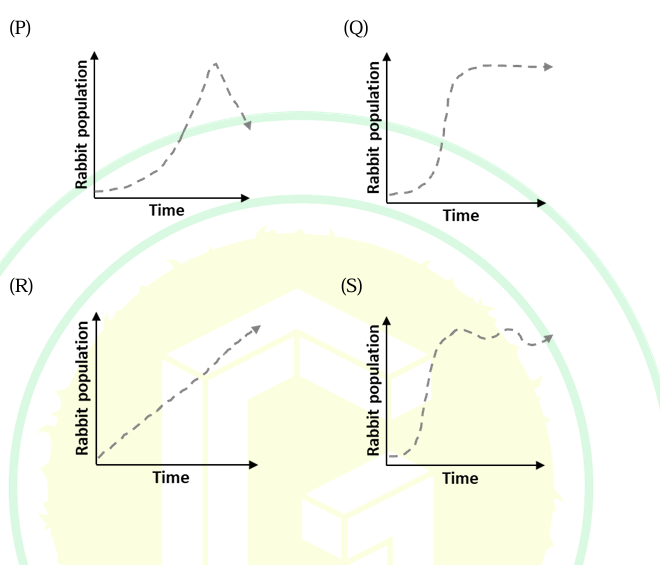
\includegraphics[width=0.8\columnwidth]{figs/xl2025_q63.png}
        \caption{Q63 que.}
    \end{figure}
    \hfill $\brak{\text{GATE XL 2025}}$
    \begin{enumerate}
        \begin{multicols}{4}
            \item P
            \item Q
            \item R
            \item S
        \end{multicols}
    \end{enumerate}

    \item Which of the following reactions in plants is/are catalyzed by the malic enzymes?

    \hfill $\brak{\text{GATE XL 2025}}$
    \begin{enumerate}
        \item Malate + NAD$^+$ $\rightarrow$ Pyruvate + CO$_2$ + NADH
        \item Malate + NAD$^+$ $=$ Oxaloacetate + NADH
        \item Malate $=$ Fumarate
        \item Malate + NADP$^+$ $\rightarrow$ Pyruvate + CO$_2$ + NADPH
    \end{enumerate}

    \item In a genetic cross between a true-breeding tall parent bearing red flowers and a true-breeding dwarf parent bearing white flowers, only tall plants with red flowers are obtained in the F$_1$ population. Considering these two traits segregate independently, if one tall individual is selected from the F$_2$ population, the probability that it would be genotypically homozygous for plant height and make red flowers is \underline{\rule{2cm}{0pt}}.

    \hfill $\brak{\text{GATE XL 2025}}$
\section*{Microbiology (XL-S)} 
\section*{Q. 66 - Q. 73 carry one mark each.} 
    \item Which one of the following metabolites is associated with bacterial stringent response?

    \hfill $\brak{\text{GATE XL 2025}}$
    \begin{enumerate}
        \begin{multicols}{2}
            \item Cyclic di-GMP $\brak{\text{CDG}}$
            \item Guanosine tetraphosphate $\brak{\text{ppGpp}}$
            \item Cyclic-AMP $\brak{\text{cAMP}}$
            \item Cyclic-GMP $\brak{\text{cGMP}}$
        \end{multicols}
    \end{enumerate}

    \item India is aiming to be free of tuberculosis by $2025$. One of the key approaches for this program is DOTS. Which one of the following options is the full form of DOTS?

    \hfill $\brak{\text{GATE XL 2025}}$
    \begin{enumerate}
        \begin{multicols}{4}
            \item Directly observed therapy short-course
            \item Directly observed tuberculosis short-course
            \item District operated therapy system
            \item Directly operated therapy short-course
        \end{multicols}
    \end{enumerate}

    \item Correctly match the bacterial type in Column I with their corresponding environmental niche in Column II.

    \begin{table}[H]
        \centering
        \begin{tabular}{ll}
            \textbf{Column I} & \textbf{Column II} \\
            P) Psychrophile & i) Pressure greater than $380$ atm \\
            Q) Barophile & ii) Temperature between $15\,^{\circ}\text{C}$ and $45\,^{\circ}\text{C}$ \\
            R) Mesophile & iii) Temperature below $15\,^{\circ}\text{C}$ \\
            S) Halophile & iv) pH less than $3.0$ \\
             & v) Salt concentration greater than $2$ M \\
        \end{tabular}
        \caption*{}
        \label{tab:xl2025_q68}
    \end{table}

    \hfill $\brak{\text{GATE XL 2025}}$
    \begin{enumerate}
        \begin{multicols}{2}
            \item P-iii; Q-i; R-ii; S-v
            \item P-ii; Q-iii; R-i; S-v
            \item P-i; Q-iv; R-iii; S-v
            \item P-v; Q-iii; R-iv; S-i
        \end{multicols}
    \end{enumerate}

    \item Robert Koch used a meat-infused nutrient medium for which one of the following purposes?

    \hfill $\brak{\text{GATE XL 2025}}$
    \begin{enumerate}
        \begin{multicols}{4}
            \item To grow disease causing microorganisms
            \item To demonstrate presence of microorganisms in air
            \item To test the efficiency of sterilization approaches
            \item To demonstrate antimicrobial activity of soil isolates
        \end{multicols}
    \end{enumerate}

    \item A penicillin sensitive \textit{Escherichia coli} population is exposed to a lethal dose $\brak{200\ \mu\text{g/mL}}$ of penicillin. Assuming density-independent mortality, which one of the following relationships would describe the number of surviving bacteria $\brak{N}$ over time $\brak{T}$?

    \hfill $\brak{\text{GATE XL 2025}}$
    \begin{enumerate}
        \begin{multicols}{4}
            \item Exponential
            \item Linear
            \item Sigmoidal
            \item parabolic
        \end{multicols}
    \end{enumerate}

    \item A bacterium obtains energy from a chemical source by the oxidation of reduced NO$_2$, with CO$_2$ as the principal carbon source. Which one of the following nutritional groups does this bacterium belong to?

    \hfill $\brak{\text{GATE XL 2025}}$
    \begin{enumerate}
        \begin{multicols}{4}
            \item Photoautotroph
            \item Photoheterotroph
            \item Chemoautotroph
            \item Chemoheterotroph
        \end{multicols}
    \end{enumerate}

    \item The origin of the \textit{Escherichia coli} chromosome on the genetic map is shown below. Bidirectional replication is a feature of this system and both replication forks move at the same rate. Which one of the following sequences of replication of the genes is correct?

    \begin{figure}[H]
        \centering
        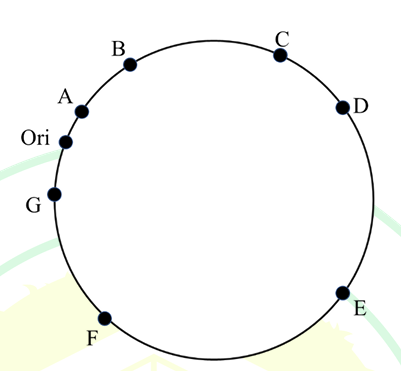
\includegraphics[width=0.8\columnwidth]{figs/xl2025_q72_que.png}
        \caption*{}
        \label{fig:xl2025_q72}
    \end{figure}

    \hfill $\brak{\text{GATE XL 2025}}$
    \begin{enumerate}
        \begin{multicols}{4}
            \item ABCDEFG
            \item AGBFCDE
            \item GAFBECD
            \item GAFEBCD
        \end{multicols}
    \end{enumerate}

    \item Which of the following sites is/are the location(s) of ATP generation through oxidative phosphorylation in \textit{Escherichia coli}?

    \hfill $\brak{\text{GATE XL 2025}}$
    \begin{enumerate}
            \item Inner membrane only
            \item Outer membrane only
            \item Both outer membrane and inner membrane
            \item Mesosome
    \end{enumerate}

\section*{Q.74 - Q.84 carry two marks each.}

    \item The adaptive immune response in an animal involves the generation of antibodies against an invading bacterial pathogen. The following graph represents antibody titer levels in a mammal exposed twice to the pathogen.
    Which one of the following options correctly pairs antibodies to peak I and peak II in the graph? 

    \begin{figure}[H]
        \centering
        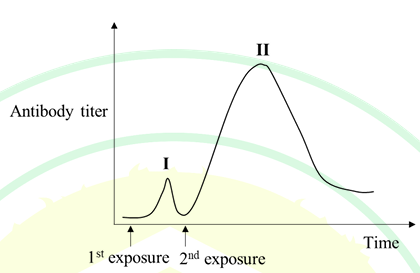
\includegraphics[width=0.7\columnwidth]{figs/xl2025_q74_que.png}
        \caption*{}
        \label{fig:xl2025_q74}
    \end{figure}

    \hfill $\brak{\text{GATE XL 2025}}$

    \begin{enumerate}
        \begin{multicols}{2}
            \item Peak I - IgG; Peak II - IgM
            \item Peak I - IgM; Peak II - IgG
            \item Peak I - IgE; Peak II - IgG
            \item Peak I - IgM; Peak II - IgE
        \end{multicols}
    \end{enumerate}

    \item Carl Woese established that short subunit rRNA sequences can be used to reveal evolutionary relationships between various organisms. Based on this, which one of the following options is the established phylogenetic arrangement of the three domains of life?

    \begin{figure}[H]
        \centering
        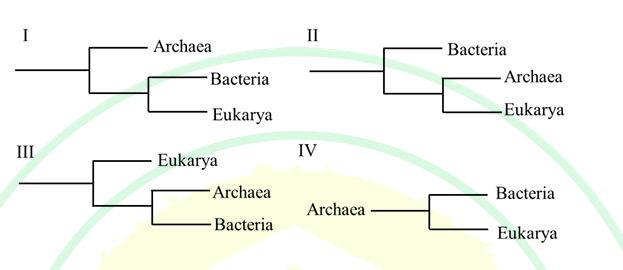
\includegraphics[width=0.7\columnwidth]{figs/xl2025_q75_que.png}
        \caption*{}
        \label{fig:xl2025_q75}
    \end{figure}

    \hfill $\brak{\text{GATE XL 2025}}$

    \begin{enumerate}
        \begin{multicols}{4}
            \item I
            \item IV
            \item II
            \item III
        \end{multicols}
    \end{enumerate}

    \item Correctly match the viruses listed in Column I with the nature of their corresponding genetic materials listed in Column II.

    \begin{table}[H]
        \centering
        \begin{tabular}{ll}
            \textbf{Column I} & \textbf{Column II} \\
            P) Bacteriophage lambda & i) dsDNA \\
            Q) Bacteriophage M13    & ii) ssDNA \\
            R) Coronavirus          & iii) ssRNA \\
            S) Reovirus             & iv) dsRNA \\
        \end{tabular}
        \caption*{}
        \label{tab:xl2025_q76}
    \end{table}

    \hfill $\brak{\text{GATE XL 2025}}$

    \begin{enumerate}
        \begin{multicols}{2}
            \item P-i; Q-iv; R-iii; S-ii
            \item P-iv; Q-ii; R-i; S-iii
            \item P-i; Q-ii; R-iii; S-iv
            \item P-i; Q-iii; R-ii; S-iv
        \end{multicols}
    \end{enumerate}

    \item A culture of lac$^+$ \textit{Escherichia coli} is grown in a medium lacking lactose or any other $\beta$-galactoside. The response of the lac operon upon induction by lactose can be monitored by measuring the levels of lac mRNA, $\beta$-galactosidase enzyme and permease enzyme. Which one of the following profiles correctly captures the on-off response to lactose?

    \begin{figure}[H]
        \centering
        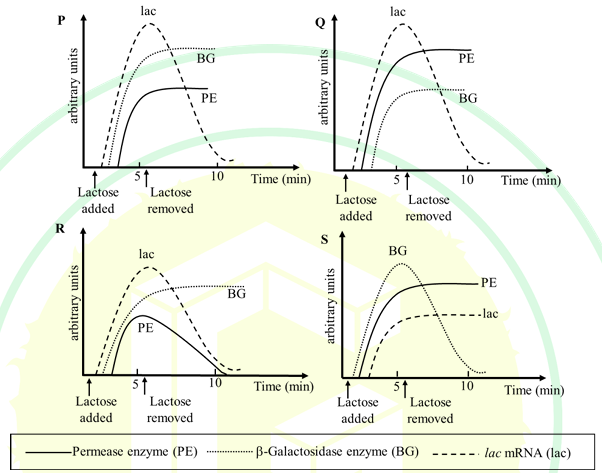
\includegraphics[width=0.9\columnwidth]{figs/xl2025_q77_que.png}
        \caption*{}
        \label{fig:xl2025_q77}
    \end{figure}

    \hfill $\brak{\text{GATE XL 2025}}$

    \begin{enumerate}
        \begin{multicols}{4}
            \item P
            \item Q
            \item R
            \item S
        \end{multicols}
    \end{enumerate}

    \item Which option(s) correctly match(es) the structures in a bacterial cell $\brak{\text{Column I}}$ with their corresponding functions $\brak{\text{Column II}}$.

    \begin{table}[H]
        \centering
        \begin{tabular}{ll}
            \textbf{Column I} & \textbf{Column II} \\
            P) Cell wall  & i) Protection from osmotic stress \\
            Q) Fimbriae   & ii) Attachment to surfaces \\
            R) Flagella   & iii) Motility \\
            S) Pili       & iv) Transfer of genetic material \\
        \end{tabular}
        \caption*{}
        \label{tab:xl2025_q78}
    \end{table}

    \hfill $\brak{\text{GATE XL 2025}}$

    \begin{enumerate}
        \begin{multicols}{2}
            \item P-i; Q-ii; R-iii; S-iv
            \item P-i; Q-iii; R-iii; S-iv
            \item P-i; Q-iv; R-ii; S-iii
            \item P-ii; Q-iv; R-i; S-iii
        \end{multicols}
    \end{enumerate}

    \item Which of the following statements regarding micro-organisms is/are correct?

    \hfill $\brak{\text{GATE XL 2025}}$

    \begin{enumerate}
        \item The free-living bacterium \textit{Wolbachia} is a human parasite.
        \item \textit{Myxococcus} are a group of predatory bacteria.
        \item \textit{Dictyostelium} is a slime mold that aggregates to form social groups.
        \item Actinomycetes in soil are involved in producing earthy odours.
    \end{enumerate}

    \item Which of the following is/are example(s) of animal-microbe mutualism?

    \hfill $\brak{\text{GATE XL 2025}}$

    \begin{enumerate}
        \item Human - \textit{Mycobacterium tuberculosis}
        \item Dog - Rabies lyssavirus
        \item Human - \textit{Lactobacillus plantarum}
        \item Cow - \textit{Methanobrevibacter ruminantium}
    \end{enumerate}

    \item Which of the following reactions is/are catalyzed by aldolase?

    \hfill $\brak{\text{GATE XL 2025}}$

    \begin{enumerate}
        \item Dihydroxyacetone phosphate + Glyceraldehyde-3-phosphate $\rightarrow$ Fructose-1,6-bisphosphate
        \item Dihydroxyacetone phosphate + Erythrose-4-phosphate $\rightarrow$ Sedoheptulose-1,7-bisphosphate
        \item Dihydroxyacetone phosphate $\rightarrow$ Glyceraldehyde-3-phosphate
        \item Glyceraldehyde-3-phosphate + Erythrose-4-phosphate $\rightarrow$ Sedoheptulose-1,7-bisphosphate
    \end{enumerate}

    \item Which option(s) correctly match(es) the Antibiotic with their corresponding Target?

    \begin{table}[H]
        \centering
        \begin{tabular}{ll}
            \textbf{Antibiotic} & \textbf{Target} \\
            P) Penicillin      & i) Ribosome \\
            Q) Kanamycin       & ii) RNA polymerase \\
            R) Rifampicin      & iii) DNA gyrase \\
            S) Nalidixic acid  & iv) Transpeptidase \\
            T) Ciprofloxacin   &  \\
        \end{tabular}
        \caption*{}
        \label{tab:xl2025_q82}
    \end{table}

    \hfill $\brak{\text{GATE XL 2025}}$

    \begin{enumerate}
        \item P-iv; Q-i; R-ii; S-iii
        \item P-ii; Q-iv; R-i; S-iii
        \item P-iv; Q-i; R-ii; T-iii
        \item P-iv; Q-iii; R-ii; T-i
    \end{enumerate}

    \item The doubling time of \textit{Escherichia coli} is $30$ minutes in a culture medium containing glucose and yeast extract. Phage T7 has a life cycle of $20$ minutes and a burst size of $200$ phage per infected \textit{E. coli} cell. Phage absorption is instantaneous and occurs at $1$ multiplicity of infection $\brak{\text{MOI}}$. Bacteria infected with multiple or single phage give the same burst. $5000$ plaque forming units of T7 phage are added to a culture of $2 \times 10^7$ \textit{E. coli} cells.\\
    Assuming normal division, the \textit{E. coli} culture will lyse completely by \underline{\rule{2cm}{0pt}} full cycles of bacterial division.

    \hfill $\brak{\text{GATE XL 2025}}$

    \item A polymerase chain reaction $\brak{\text{PCR}}$ based diagnosis test was performed on a bacterial sample targeting a specific gene. There are $3$ copies of this gene in the bacterial genome. Prior to DNA extraction, the bacteria were incubated to allow one cycle of growth. $3072$ amplicon copies were obtained after $9$ cycles of the PCR. Assume $100\%$ efficiency at each step.\\
    The initial bacterial count in the sample was \underline{\rule{2cm}{0pt}}.

    \hfill $\brak{\text{GATE XL 2025}}$

\section*{Zoology (XL-T)}
\section*{Q.85 - Q.92 carry one mark each.}

    \item Which one of the following is a ``brood parasite''?

    \hfill $\brak{\text{GATE XL 2025}}$
    \begin{enumerate}
        \begin{multicols}{4}
            \item Pigeon
            \item Sparrow
            \item Goose
            \item Cuckoo
        \end{multicols}
    \end{enumerate}

    \item During the development of a mammalian embryo, ``yolk sac'' is formed by which one of the following?

    \hfill $\brak{\text{GATE XL 2025}}$
    \begin{enumerate}
        \begin{multicols}{4}
            \item Syncytiotrophoblast
            \item Primitive endoderm $\brak{\text{hypoblast}}$
            \item Amniotic ectoderm
            \item Embryonic epiblast
        \end{multicols}
    \end{enumerate}

    \item The animals belonging to which one of the following phyla are characterized by ``segmented body''?

    \hfill $\brak{\text{GATE XL 2025}}$
    \begin{enumerate}
        \begin{multicols}{2}
            \item Annelida
            \item Cnidaria
            \item Echinodermata
            \item Porifera
        \end{multicols}
    \end{enumerate}

    \item Which one of the following is a ``post-zygotic'' isolating mechanism of speciation?

    \hfill $\brak{\text{GATE XL 2025}}$
    \begin{enumerate}
        \begin{multicols}{2}
            \item Behavioral isolation
            \item Fertilization failure
            \item Hybrid sterility
            \item Seasonal isolation
        \end{multicols}
    \end{enumerate}

    \item Desmosomes are

    \hfill $\brak{\text{GATE XL 2025}}$
    \begin{enumerate}
            \item Intermediate filament-based cell adhesion complexes
            \item Protein synthesizing macromolecular complexes
            \item Subcellular organelles
            \item DNA-protein complexes
    \end{enumerate}

    \item The ``foramen of Panizza'' is found in which one of the following groups of animals?

    \hfill $\brak{\text{GATE XL 2025}}$
    \begin{enumerate}
        \begin{multicols}{4}
            \item Fishes
            \item Crocodiles
            \item Frogs
            \item Dolphins
        \end{multicols}
    \end{enumerate}

    \item Imagine a population of diploid species in Hardy-Weinberg equilibrium. The population has two alleles for a gene which are $a$ and $A$. The number of individuals with $aa$ genotype in this population is $1$ in $10000$. The frequency of the allele $A$ in the population is \underline{\rule{2cm}{0pt}} $\brak{\text{up to two decimal places}}$.

    \hfill $\brak{\text{GATE XL 2025}}$

    \item A PCR was set up to amplify a $500$ nucleotides-long DNA. The dNTPs in the reaction mixture were radiolabeled. The percentage of radiolabeled single-stranded DNA after three cycles will be \underline{\rule{2cm}{0pt}} $\brak{\text{up to one decimal place}}$.

    \hfill $\brak{\text{GATE XL 2025}}$

\section*{Q.93 - Q.103 carry two marks each.}

    \item Match the molecules in Column-I with their properties/functions mentioned in Column-II.

    \begin{table}[H]
        \centering
        \begin{tabular}{ll}
            \textbf{Column-I} & \textbf{Column-II} \\
            P) IgM  & 1) Involved in antigen presentation \\
            Q) IgE  & 2) Predominant antibody type in various body secretions \\
            R) IgA  & 3) Can pass through placenta \\
            S) MHC  & 4) Associated with allergic reaction \\
                    & 5) Contains ten heavy and light chains \\
        \end{tabular}
        \caption*{}
        \label{tab:xl2025_q93}
    \end{table}

    \hfill $\brak{\text{GATE XL 2025}}$
    \begin{enumerate}
        \begin{multicols}{2}
            \item P-3; Q-2; R-4; S-5
            \item P-5; Q-4; R-2; S-1
            \item P-2; Q-3; R-4; S-1
            \item P-4; Q-1; R-3; S-5
        \end{multicols}
    \end{enumerate}

    \item Match the following human diseases in Column-I with their causal organism in Column-II.

    \begin{table}[H]
        \centering
        \begin{tabular}{ll}
            \textbf{Column-I} & \textbf{Column-II} \\
            P) Sleeping sickness & 1) \textit{Trypanosoma cruzi} \\
            Q) Chagas disease    & 2) \textit{Trypanosoma brucei} \\
            R) Elephantiasis     & 3) \textit{Borrelia burgdorferi} \\
            S) Lyme disease      & 4) \textit{Wuchereria bancrofti} \\
                                 & 5) \textit{Rickettsia rickettsii} \\
        \end{tabular}
        \caption*{}
        \label{tab:xl2025_q94}
    \end{table}

    \hfill $\brak{\text{GATE XL 2025}}$
    \begin{enumerate}
        \begin{multicols}{2}
            \item P-3; Q-1; R-4; S-5
            \item P-1; Q-2; R-3; S-4
            \item P-2; Q-4; R-1; S-3
            \item P-2; Q-1; R-4; S-3
        \end{multicols}
    \end{enumerate}

    \item Match the molecules in Column-I with their correct property/function in Column-II.

    \begin{table}[H]
        \centering
        \begin{tabular}{ll}
            \textbf{Column-I} & \textbf{Column-II} \\
            P) RNase P        & 1) rRNA gene transcription \\
            Q) RNA Polymerase-I & 2) Gene silencing \\
            R) siRNA          & 3) Cas9-mediated genome editing \\
            S) Guide RNA      & 4) Ribozymes \\
                              & 5) tRNA gene transcription \\
        \end{tabular}
        \caption*{}
        \label{tab:xl2025_q95}
    \end{table}

    \hfill $\brak{\text{GATE XL 2025}}$
    \begin{enumerate}
        \begin{multicols}{2}
            \item P-4; Q-5; R-2; S-3
            \item P-5; Q-1; R-3; S-4
            \item P-4; Q-1; R-2; S-3
            \item P-5; Q-4; R-1; S-2
        \end{multicols}
    \end{enumerate}

    \item What would be the number of genotypes and phenotypes, respectively, from a cross between genotypes AaBBCcDd and AaBBCcDd? Assume independent assortment and simple dominant-recessive relationship in each gene pair.

    \hfill $\brak{\text{GATE XL 2025}}$
    \begin{enumerate}
        \begin{multicols}{2}
            \item 8 and 4
            \item 12 and 4
            \item 27 and 8
            \item 14 and 8
        \end{multicols}
    \end{enumerate}

    \item Nucleosomes are made up of DNA and histones. Histones undergo various kinds of modifications by different groups of proteins. They are known as histone writers, readers and erasers. Which of the following is/are histone writer(s)?

    \hfill $\brak{\text{GATE XL 2025}}$
    \begin{enumerate}
        \item Histone acetyl transferases
        \item Histone methyl transferases
        \item Histone deacetylases
        \item DNA methyl transferases
    \end{enumerate}

    \item The expression of a gene is regulated by a transcription factor. Which of the following techniques can be used to identify the region in its promoter where the transcription factor binds?

    \hfill $\brak{\text{GATE XL 2025}}$
    \begin{enumerate}
        \item S1 nuclease mapping
        \item Chromatin immunoprecipitation followed by sequencing
        \item Electrophoretic mobility shift assay
        \item DNase I footprinting
    \end{enumerate}

    \item Which of the following animals in India are included under ``critically endangered'' threat category as per the Red Data List of IUCN?

    \hfill $\brak{\text{GATE XL 2025}}$
    \begin{enumerate}
        \item Namdapha Flying Squirrel
        \item Indian Rhinoceros
        \item Nicobar Shrew
        \item Clouded Leopard
    \end{enumerate}

    \item Which of the following statements in relation to cell movement during gastrulation in Sea urchin is/are correct?

    \hfill $\brak{\text{GATE XL 2025}}$
    \begin{enumerate}
        \item Delamination leads to the formation of endoderm
        \item Ingression leads to the development of mesoderm
        \item Involution leads to the development of ectoderm
        \item Invagination leads to the development of endoderm
    \end{enumerate}

    \item Which of the following genetic disorders is/are caused by trinucleotide repeat expansions?

    \hfill $\brak{\text{GATE XL 2025}}$
    \begin{enumerate}
        \item Huntington's disease
        \item $\beta$-thalassemia
        \item Fragile X syndrome
        \item Cystic fibrosis
    \end{enumerate}

    \item The mother and the father of five children are carriers (heterozygous) of an autosomal recessive allele that causes cystic fibrosis. The probability of having exactly three normal children among five is \underline{\rule{2cm}{0pt}}.

    \hfill $\brak{\text{GATE XL 2025}}$

    \item An enzyme, which follows Michaelis-Menten equation, catalyzes the reaction A $\rightarrow$ B. When enzyme and substrate concentrations are $15$nM and $10\,\mu$M, respectively, the reaction velocity is $5\,\mu$Ms$^{-1}$. If $K_m$ for the substrate A is $5\,\mu$M, the kinetic efficiency of the enzyme will be $\times 10^6$M$^{-1}$s$^{-1}$ \underline{\rule{2cm}{0pt}}.

    \hfill $\brak{\text{GATE XL 2025}}$

\section*{Food Technology (XL-U)} 
\section*{Q.104 - Q.111 carry one mark each.}

    \item Which of the following contains the phytonutrient allicin?

    \hfill $\brak{\text{GATE XL 2025}}$
    \begin{enumerate}
        \begin{multicols}{4}
            \item Grape
            \item Cauliflower
            \item Garlic
            \item Chilli
        \end{multicols}
    \end{enumerate}

    \item Which mold is responsible for the characteristic blue marbling in blue-veined cheese?

    \hfill $\brak{\text{GATE XL 2025}}$
    \begin{enumerate}
        \begin{multicols}{2}
            \item \textit{Rhizopus oryzae}
            \item \textit{Penicillium roqueforti}
            \item \textit{Aspergillus niger}
            \item \textit{Penicillium camemberti}
        \end{multicols}
    \end{enumerate}

    \item Which genus of bacteria does NOT have cell wall?

    \hfill $\brak{\text{GATE XL 2025}}$
    \begin{enumerate}
        \begin{multicols}{4}
            \item \textit{Lactobacillus}
            \item \textit{Staphylococcus}
            \item \textit{Mycoplasma}
            \item \textit{Escherichia}
        \end{multicols}
    \end{enumerate}

    \item Which of the following pigments does NOT have pro-vitamin A activity?

    \hfill $\brak{\text{GATE XL 2025}}$
    \begin{enumerate}
        \begin{multicols}{2}
            \item $\beta$-Carotene
            \item $\beta$-Cryptoxanthin
            \item Lycopene
            \item $\alpha$-Carotene
        \end{multicols}
    \end{enumerate}

    \item Identify the analysis that must be performed FIRST to judge cleanliness of spice/herb powders.

    \hfill $\brak{\text{GATE XL 2025}}$
    \begin{enumerate}
        \begin{multicols}{2}
            \item Acid-insoluble ash content
            \item Pesticide residue levels
            \item Volatile oil content
            \item Mycotoxin levels
        \end{multicols}
    \end{enumerate}

    \item If there is a delay in oil extraction after bran is separated from the brown rice, the quality of rice bran oil deteriorates. Identify the suitable CAUSE and EFFECT for the deterioration in oil quality.

    \hfill $\brak{\text{GATE XL 2025}}$
    \begin{enumerate}
        \item Lipase activity; increase in FFA
        \item Oil hydrolysis; decrease in FFA
        \item Lipase activity; decrease in FFA
        \item Bran stabilization; decrease in lipase activity
    \end{enumerate}

    \item Among the following, which is/are the process(es) that lead to generation of new fats from existing ones?

    \hfill $\brak{\text{GATE XL 2025}}$
    \begin{enumerate}
        \item Transesterification
        \item Degumming
        \item Hydrogenation
        \item Winterization
    \end{enumerate}

\section*{Q.111 - Q.122 carry two marks each.}

    \item The true density and bulk density of wheat grains are $1280\ \text{kg/m}^3$ and $740\ \text{kg/m}^3$, respectively.  
    The porosity of the grains is \underline{\rule{2cm}{0pt}} $\brak{\text{rounded off to 2 decimal places}}$.

    \hfill $\brak{\text{GATE XL 2025}}$

    \item Identify the gas composition $\brak{\text{in percent}}$ suitable for packaging cured meat under MAP conditions.

    \hfill $\brak{\text{GATE XL 2025}}$
    \begin{enumerate}
        \begin{multicols}{2}
            \item O$_2$ = $0$; CO$_2$ = $50$; N$_2$ = $50$
            \item O$_2$ = $50$; CO$_2$ = $0$; N$_2$ = $50$
            \item O$_2$ = $0$; CO$_2$ = $0$; N$_2$ = $100$
            \item O$_2$ = $50$; CO$_2$ = $50$; N$_2$ = $0$
        \end{multicols}
    \end{enumerate}

    \item Which of the following sequence of events occurs during formation of egg-white gel?\\
    Assume: PN = Native protein; PD = Denatured protein; PA = Aggregated protein; PG = Protein gel; $\rightarrow$ = forward reaction; $\leftrightarrow$ = reversible reaction; $\Delta$ = heating; $\nabla$ = cooling.

    \hfill $\brak{\text{GATE XL 2025}}$
    \begin{enumerate}
        \item $\Delta$ PN $\rightarrow$ PD $\rightarrow$ PA $\rightarrow$ PG
        \item PN $\rightarrow$ PD $\rightarrow$ PG
        \item $\Delta$ PN $\rightarrow$ PD $\rightarrow$ PG
        \item $\Delta$ PN $\rightarrow$ PA $\rightarrow$ PG
    \end{enumerate}

    \item In canning and retorting of foods, which of the following is the correct expression of Ball process time $\brak{B}$?\\
    Assume: $t_p$ = processor's process time; $t_c$ = come-up time.

    \hfill $\brak{\text{GATE XL 2025}}$
    \begin{enumerate}
        \begin{multicols}{2}
            \item $B = t_p + 0.42\, t_c$
            \item $B = t_p + 0.30\, t_c$
            \item $B = t_p + 0.50\, t_c$
            \item $B = t_p + 0.25\, t_c$
        \end{multicols}
    \end{enumerate}

    \item Which of the following is the most suitable flexible packaging laminate for dry fruits?

    \hfill $\brak{\text{GATE XL 2025}}$
    \begin{enumerate}
        \begin{multicols}{2}
            \item PET/LDPE
            \item PS/LDPE
            \item OPP/LDPE
            \item Nylon/LDPE
        \end{multicols}
    \end{enumerate}

    \item Identify the CORRECT sequence of operations for dressing of poultry.

    \hfill $\brak{\text{GATE XL 2025}}$
    \begin{enumerate}
        \item Slaughtering and bleeding $\rightarrow$ scalding $\rightarrow$ defeathering $\rightarrow$ eviscerating $\rightarrow$ chilling
        \item Slaughtering and bleeding $\rightarrow$ defeathering $\rightarrow$ scalding $\rightarrow$ eviscerating $\rightarrow$ chilling
        \item Slaughtering and bleeding $\rightarrow$ eviscerating $\rightarrow$ defeathering $\rightarrow$ scalding $\rightarrow$ chilling
        \item Slaughtering and bleeding $\rightarrow$ defeathering $\rightarrow$ eviscerating $\rightarrow$ scalding $\rightarrow$ chilling
    \end{enumerate}

    \item Which of the following statement(s) is/are TRUE for a package of gamma-irradiated $\brak{7.5\ \text{kGy}}$ whole chicken?

    \hfill $\brak{\text{GATE XL 2025}}$
    \begin{enumerate}
        \item Nutritional quality of the product deteriorates after irradiation.
        \item Spores of \textit{C. botulinum} can survive in the irradiated product.
        \item 'Radura' symbol does not ensure safety of the irradiated product for consumption.
        \item Energy needed for the irradiation process is much higher than that required for freezing of the product.
    \end{enumerate}

    \item Match the following food products in Column-I with their corresponding processes in Column-II.

    \begin{table}[H]
        \centering
        \begin{tabular}{ll}
            \textbf{Column-I} & \textbf{Column-II} \\
            P) Idli & 1) Baking \\
            Q) Parboiled rice & 2) Fermentation \\
            R) Soda beverage & 3) Gelatinization \\
            S) Cookies & 4) Carbonation \\
        \end{tabular}
        \caption*{}
        \label{tab:xl2025_q118}
    \end{table}

    \hfill $\brak{\text{GATE XL 2025}}$
    \begin{enumerate}
        \begin{multicols}{2}
            \item P-2; Q-3; R-4; S-1
            \item P-3; Q-2; R-4; S-1
            \item P-2; Q-4; R-1; S-3
            \item P-2; Q-3; R-1; S-4
        \end{multicols}
    \end{enumerate}

    \item Which one of the following is used as a chelating agent in foods?

    \hfill $\brak{\text{GATE XL 2025}}$
    \begin{enumerate}
        \begin{multicols}{4}
            \item Citric acid
            \item EDTA
            \item Mannitol
            \item Ascorbic acid
        \end{multicols}
    \end{enumerate}

    \item Match the following enzymes in Column-I with their applications in Column-II.

    \begin{table}[H]
        \centering
        \begin{tabular}{ll}
            \textbf{Column-I} & \textbf{Column-II} \\
            P) $\beta$-Glucanase & 1) Fruit juice clarification \\
            Q) $\alpha$- and $\beta$-Amylases & 2) Bread making \\
            R) Pectinase & 3) Meat tenderization \\
            S) Papain & 4) Brewing \\
        \end{tabular}
        \caption*{}
        \label{tab:xl2025_q120}
    \end{table}

    \hfill $\brak{\text{GATE XL 2025}}$
    \begin{enumerate}
        \begin{multicols}{2}
            \item P-3; Q-1; R-2; S-4
            \item P-4; Q-2; R-1; S-3
            \item P-2; Q-4; R-1; S-3
            \item P-1; Q-2; R-3; S-4
        \end{multicols}
    \end{enumerate}

    \item The $F_{121}$ value of a known microorganism with $Z$ value of $11\ ^\circ\text{C}$ is $2.4$min for $99.9999\%$ inactivation. For a 12D inactivation of the said microorganism at $143\ ^\circ\text{C}$, the $F$ value (in min) is \underline{\rule{2cm}{0pt}} $\brak{\text{rounded off to 3 decimal places}}$.

    \hfill $\brak{\text{GATE XL 2025}}$

   \item In a typical grinding operation, $80\%$ of the feed material passes through a sieve opening of $4.75$mm; whereas, $80\%$ of the ground product passes through $0.5$mm opening. If the power required to grind $2$tonnes/h of the feed material is $3.8$kW, the work index of the material is \underline{\rule{2cm}{0pt}} $\brak{\text{rounded off to 2 decimal places}}$.\hfill $\brak{\text{GATE XL 2025}}$

\end{enumerate}
\end{document}